% Chapter Template

\chapter{Υλοποίηση} % Main chapter title

\label{Υλοποίηση} % Change X to a consecutive number; for referencing this chapter elsewhere, use \ref{ChapterX}

\lhead{Κεφάλαιο 4. \emph{Υλοποίηση}} % Change X to a consecutive number; this is for the header on each page - perhaps a shortened title
\noindent
Σε αυτό το κεφάλαιο θα γίνει μια ανασκόπηση της υλοποίησης του \setlanguage{english} socialpserver \setlanguage{greek}, θα περιγραφούν ο java κώδικας, οι διαφορετικές κλάσεις και οι μέθοδοι που αναπτύχθηκαν.
Οι κλάσεις που χρησιμοποιούνται είναι χωρισμένες στα εξής πακέτα.


\begin{description}
\item \textbf{  \hyperref[socialpserver]{ socialpserver   \ref*{socialpserver} } }  \hfill \\
Το οποίο περιλαμβάνει τις βασικότερες για την λειτουργία, κλάσεις του socialPServer.
\item \textbf{ \hyperref[socialpserver.algorithmic]{ socialpserver.algorithmic   \ref*{socialpserver.algorithmic} }  }  \hfill \\
Στο οποίο βρίσκονται κλάσεις σχετικές με τους αλγορίθμους που χρησιμοποιούνται για την παραγωγή communities.
\item \textbf{  \hyperref[socialpserver.dataio]{ socialpserver.dataio   \ref*{socialpserver.dataio} }  }   \hfill \\
Που περιλαμβάνει όλες τις κλάσεις που σχετίζονται με την είσοδο και έξοδο Δεδομένων. 
\end{description}


\section{Πακέτο socialpserver}
\label{socialpserver}
\noindent
To πακέτο αυτό περιλαμβάνει τα δομικά εργαλεία του project. Εδώ βρίσκονται οι κλάσεις που περιγράφουν τις δομές δεδομένων οι οποίες θα αντιπροσωπεύσουν τα αποτελέσματα,
δηλαδή τα communities χρηστών καθώς και η main method. Εδώ επίσης έχουν τοποθετηθεί ως υπο-πακέτα τα υπολειπόμενα πακέτα της εφαρμογής: \emph{.algorithmic} και \emph{.dataio} \\
συγκεκριμένα εμπεριέχονται οι κλάσεις:

\begin{itemize}
\renewcommand{\labelitemi}{$\star$}
\item \textbf{  \hyperref[main]{ SocialSPerver-main   \ref*{main} } } 
\item \textbf{  \hyperref[Community]{ Community   \ref*{Community} }  }  
\item \textbf{  \hyperref[SetOfCommunities]{ SetOfCommunities   \ref*{SetOfCommunities} }  } 
\end{itemize}


\begin{figure}[htbp]
  %\begin{center}
  \hspace{-3.0em}    
    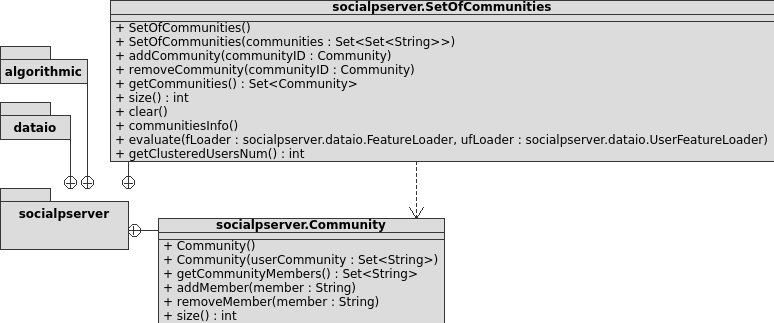
\includegraphics[scale=0.80]{Figures/socialpserverPackageClassDiagram.png}
	\rule{35em}{0.5pt}  % UnderLine figure	
	\caption[socialPServerClassDiagram]{socialPServer Package classDiagram}
  %\end{center}	
  \label{fig:socialPServerClassDiagram}  
\end{figure}


\subsection{SocialPServer-main}
\label{main}
\noindent
Εδώ βρίσκεται και η μέθοδος \textbf{main} η οποία ταξινομεί τις λειτουργίες του προγράμματος. Σε πρώτο στάδιο η main καλείται να κάνει τις απαραίτητες αρχικοποιήσεις 
επομένως δημιουργεί την αρχική σύνδεση με την Βάση Δεδομένων την οποία θα χρησιμοποιήσουν οι ακόλουθες λειτουργίες και αρχικοποιεί τους \emph{Loggers} ώστε να διαχειρίζονται
με αποδοτικό τρόπο τα μηνύματα εξόδου. Στη συνέχεια δημιουργεί τους \emph{DataLoaders} που θα αναλάβουν το πέρασμα των απαραίτητων δεδομένων και ανάλογα με την λειτουργία
που πρέπει να εκτελεστεί καλεί τους αλγορίθμους να παράξουν κοινότητες. Τέλος διαχειρίζεται την έξοδο αυτών αποθηκεύοντας την παραγόμενη πληροφορία ή καλώντας 
την αξιολόγηση των αποτελεσμάτων.

Στην βασική αυτή κλάση ακόμα περιλαμβάνεται και η μέθοδος \textbf{socialUtils} η οποία παρέχει τις αρχικές πληροφορίες για τον κοινωνικό γράφο,
πράγμα που βελτιώνει την λειτουργικότητα καθώς οι πληροφορίες αυτές είναι χρήσιμες τόσο για τον προγραμματιστή
αλλά και για τον διαχειριστή της εκάστοτε υπηρεσίας, αφού εδώ γίνονται γνωστά χαρακτηριστικά όπως το πλήθος των χρηστών και των ακμών φιλίας.


\subsection{Community}
\label{Community}
\noindent
Σε αυτό το σημείο θα περιγραφεί τι πραγματικά σημαίνει κοινότητα χρηστών (community) για τον πρόγραμμά μας.
Για να μπορεί ο socialPServer να αντιληφθεί και να χειριστεί μια κοινότητα έχει υλοποιηθεί η κλάση \textbf{Community}
η οποία είναι η Δομή Δεδομένων που αντιπροσωπεύει μια τέτοια ομάδα χρηστών.
Επομένως για κάθε παραγόμενη κοινότητα δημιουργούμε ένα νέο αντικείμενο αυτής της κλάσης και του περνάμε τις απαραίτητες πληροφορίες.

Ποιο αναλυτικά, η βάση μιας κοινότητας είναι ένα \textbf{java HashSet} που περιλαμβάνει userIDs.
Ένα java Set είναι ιδανικό για να περιγράψει μια κοινότητα αφού, θέλουμε τα μέλη να είναι μοναδικά (\emph{unique}) 
και δεν μας απασχολεί η σειρά με την οποία είναι αποθηκευμένα (\emph{unordered}).
Επίσης επιλέχθηκε συγκεκριμένα HashSet γιατί είναι η πιο αποδοτική δομή για τον χειρισμό τέτοιου είδους δεδομένων σε επίπεδο πόρων.\\
Με αυτήν την κλάση μπορούμε να προσθέσουμε τις επιπλέον λειτουργίες που χρειάζεται το πρόγραμμα καθώς και να προστατεύσουμε τη δομή από τη χρήση λειτουργιών των java Sets που
δεν χρειάζονται στην προκειμένη περίπτωση και θα ήταν εν δυνάμει καταστροφικές. Ουσιαστικά έτσι δημιουργείται ένα 'υψηλότερο' επίπεδο χειρισμού δεδομένων αφού οι διάφορες μέθοδοι
αλληλεπιδρούν με την κοινότητα μέσω αυτής της κλάσης.

Εμπεριέχεται μία global μεταβλητή:
\begin{lstlisting}[frame=single]  % Start your code-block

  private Set<String> community;
\end{lstlisting}


Αρχικά, με την δημιουργία ενός τέτοιου αντικειμένου ενεργοποιείται ο  \setlanguage{english} \textbf{constructor} \setlanguage{greek} που μπορεί να πάρει δύο μορφές, ανάλογα με το input που δίνεται.\\
Στην πρώτη περίπτωση μπορεί να δημιουργήσει κανείς ένα τέτοιο αντικείμενο χωρίς να δώσει κάποια παράμετρο
γράφοντας:

\begin{lstlisting}[frame=single]  % Start your code-block

  Community comID = new Community();
\end{lstlisting}
 
  
  όπου ο \emph{constructor} αρχικοποιεί το \emph{global community} με αυτόν τον τρόπο:
  
\begin{lstlisting}[frame=single]  % Start your code-block

  public Community() {
    this.community = new HashSet<>();
  }
\end{lstlisting}
 

  ή σε άλλη περίπτωση μπορεί από την πρώτη στιγμή να δώσει και το περιεχόμενο της δομής γράφοντας:
\begin{lstlisting}[frame=single]  % Start your code-block

  Community comID  = new Community(algorithm.out.comID);
\end{lstlisting}

 
  
  όπου ο \emph{constructor} αρχικοποιεί το \emph{global community} κάνοντας:
  
\begin{lstlisting}[frame=single]  % Start your code-block

  public Community(Set<String> userCommunity) {
        this.community = new HashSet<>();
        for (String user : userCommunity) {
            community.add(user);
        }
  }
\end{lstlisting}
  


Αφού αρχικοποιηθεί λοιπόν η δομή, ο δημιουργός του αντικειμένου πρέπει να μπορεί να εκτελέσει 'χαμηλότερου' επιπέδου λειτουργίες αλληλεπίδρασης. Υλοποιήθηκαν επομένως οι παρακάτω
μέθοδοι:


\begin{description}
\item \textbf{addMember}  \hfill \\
  πρόσθεση μέλους στην κοινότητα
\begin{lstlisting}[frame=single]  % Start your code-block

  community.add(member);
\end{lstlisting}
\item \textbf{removeMember}  \hfill \\
  αφαίρεση μέλους από την κοινότητα
\begin{lstlisting}[frame=single]  % Start your code-block

  community.remove(member);
\end{lstlisting}
\item \textbf{getCommunityMembers}   \hfill \\
  ανάκτηση μελών της κοινότητας
\begin{lstlisting}[frame=single]  % Start your code-block

  return community;
\end{lstlisting}
\item \textbf{size}   \hfill \\
  μέγεθος της κοινότητας
\begin{lstlisting}[frame=single]  % Start your code-block

  return community.size();
\end{lstlisting}
\end{description}



Τέλος, εδώ βρίσκονται κάποιες μέθοδοι που εμπλέκονται στην διαδικασία αξιολόγησης της παραγωγής κοινοτήτων δίνοντας σχετικές πληροφορίες, οι οποίες θα αναλυθούν
στο κεφάλαιο \textbf{\hyperref[eval]{Εvaluation 5.3} }.


\subsection{SetOfCommunities}
\label{SetOfCommunities}
\noindent
Ο κάθε αλγόριθμος πρόκειται να παράξει ένα σύνολο communities επομένως προκύπτει η ανάγκη δημιουργίας μιας δομής που θα
μπορεί να χειριστεί ένα τέτοιο σύνολο. Έτσι υλοποιήθηκε η κλάση \textbf{SetOfCommunities}.

Η δομή αυτή όπως προκύπτει και από το όνομά της βασίζεται σε ένα \emph{global java HashSet} που περιλαμβάνει
αντικείμενα τύπου \emph{Community}.\\
\begin{lstlisting}[frame=single]  % Start your code-block

  private Set<Community> communities;
\end{lstlisting}

Και σε αυτήν την περίπτωση η δημιουργία ενός τέτοιου αντικειμένου μπορεί να πάρει δύο μορφές, αναλόγως με την μορφή
του \emph{constructor} που θα υιοθετήσουμε. \\

  
Στην πρώτη περίπτωση μπορεί να δημιουργήσει κανείς ένα τέτοιο αντικείμενο χωρίς να δώσει κάποια παράμετρο: 


\begin{lstlisting}[frame=single]  % Start your code-block

  SetOfCommunities comSet = new SetOfCommunities();
\end{lstlisting}
 
  
  όπου ο \emph{constructor} αρχικοποιεί το \emph{global Set<Community> communities} με αυτόν τον τρόπο:
  
\begin{lstlisting}[frame=single]  % Start your code-block

  public SetOfCommunities() {
      this.communities = new HashSet<>();
  }
\end{lstlisting}
 
  ή σε κάποια άλλη μπορεί από την πρώτη στιγμή να δώσει και το περιεχόμενο της:
\begin{lstlisting}[frame=single]  % Start your code-block

  SetOfCommunities comSet = new SetOfCommunities(algorithm.out);
\end{lstlisting}

   
  όπου ο \emph{constructor} αρχικοποιεί το \emph{global Set<Community> communities} κάνοντας:
  
\begin{lstlisting}[frame=single]  % Start your code-block

    public SetOfCommunities(Set<Set<String>> communities) {
        this.communities = new HashSet<>();
        for (Set<String> community : communities) {
            this.communities.add(new Community(community));            
        }
    }
\end{lstlisting}
  
 
Όπως και προηγουμένως έτσι και σε αυτήν στην δομή μετά την αρχικοποίηση πρέπει να δίνονται στον προγραμματιστή
κάποιες βασικές λειτουργίες για τον χειρισμό αυτού του Set.
Υλοποιήθηκαν επομένως οι παρακάτω μέθοδοι:

\begin{description}
\item \textbf{addCommunity}  \hfill \\
  πρόσθεση κοινότητας στο Set
\begin{lstlisting}[frame=single] 
  communities.add(communityID);
\end{lstlisting}
\item \textbf{removeCommunity}  \hfill \\
  αφαίρεση κοινότητας από το Set
\begin{lstlisting}[frame=single]
  communities.remove(communityID);
\end{lstlisting}
\item \textbf{getCommunities}   \hfill \\
  ανάκτηση όλων των κοινοτήτων
\begin{lstlisting}[frame=single] 
  return communities;
\end{lstlisting}
\item \textbf{size}   \hfill \\
  πλήθος των κοινοτήτων
\begin{lstlisting}[frame=single]
  return communities.size();
\end{lstlisting}
\item \textbf{clear}   \hfill \\
  finalize, free memory. Διαγραφή όλων των κοινοτήτων για ελευθέρωση της μνήμης και επίσης διαγραφή των υπόλοιπων δομών που περιέχουν δεδομένα
\begin{lstlisting}[frame=single] 
    public void clear() {
        if (communities.size()>0) {
            communities.clear();
        }
        if (allCentroidFeatures.size()>0) {
            allCentroidFeatures.clear();
        }
    }
\end{lstlisting}  
\end{description}  
  
Επίσης για μία συνολική ανασκόπηση των κοινοτήτων υπάρχει η μέθοδος:  
\begin{description}  
\item \textbf{communitiesInfo}   \hfill \\
  η οποία δίνει γενικές πληροφορίες όπως:\\
  \textbf{maxCommunitySize, minCommunitySize, averageCommunitySize, κτλ}\\
  (συνήθως καλείται αμέσως πριν την διαδικασία Evaluation αλλά μπορεί να καλεστεί και οποιαδήποτε άλλη στιγμή
\end{description}


Τέλος εδώ βρίσκονται κάποιες μέθοδοι που εμπλέκονται στην διαδικασία αξιολόγησης \textbf{\hyperref[eval]{Εvaluation 5.3} }, οι οποίες θα αναλυθούν
στο σχετικό κεφάλαιο.


\section{Πακέτο socialpserver.algorithmic}
\label{socialpserver.algorithmic}
\noindent
Εδώ περιγράφονται οι κλάσεις που αφορούν τους αλγορίθμους που χρησιμοποιούνται για την παραγωγή κοινοτήτων.\\

Όπως αναφέρθηκε και στο κεφάλαιο \textbf{~\ref{Αλγόριθμοι}}  η εξαγωγή κοινοτήτων χρηστών 
μπορεί να γίνει με πολλούς διαφορετικούς τρόπους.
Χρησιμοποιήθηκε ένας αριθμός αλγορίθμων που  που έχουν χρησιμότητα για την δικιά μας περίπτωση 
οι οποίοι είναι δανεισμένοι από java βιβλιοθήκες ανοιχτού κώδικα.


\begin{figure}[htbp]
  %\begin{center}
  \hspace{-4.0em}    
    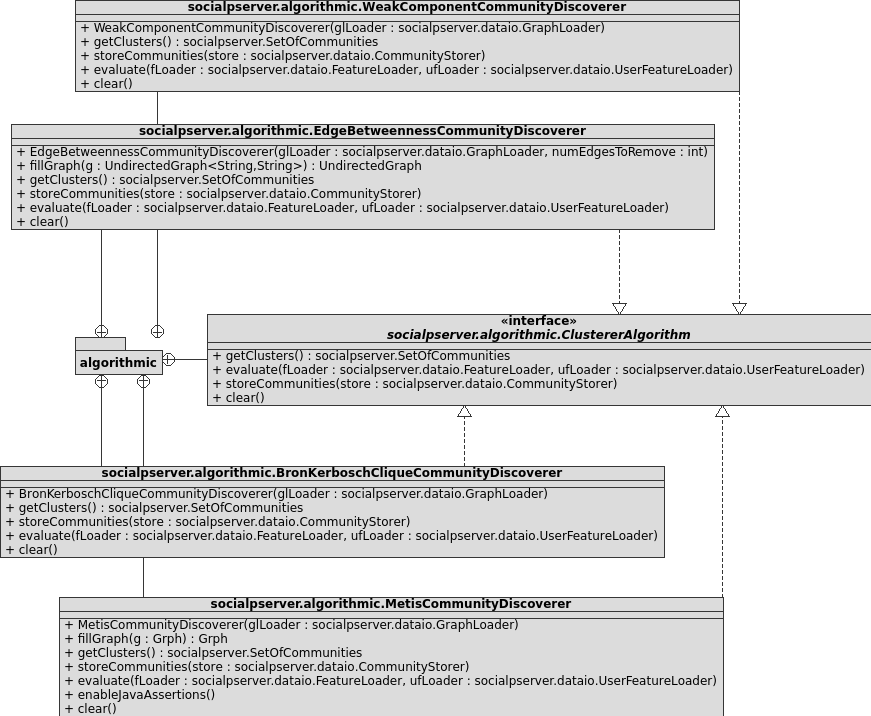
\includegraphics[scale=0.80]{Figures/algorithmicClassDiagram.png}
	\rule{35em}{0.5pt}  % UnderLine figure	
	\caption[algorithmicClassDiagram]{.algorithmic Package classDiagram}
  %\end{center}	
  \label{fig:algorithmicClassDiagram}  
\end{figure}



\subsection{interface ClustererAlgorithm}
\noindent
Αφού γίνεται χρήση αλγορίθμων που ανήκουν σε διαφορετικές βιβλιοθήκες, είναι φανερό πως πρέπει το πρόγραμμα να είναι σχεδιασμένο με τέτοιο τρόπο 
ώστε να υποστηρίζει την πρόσθεση και αφαίρεση αλγορίθμων και λειτουργιών. Πρέπει δηλαδή στην υλοποίηση να είναι ξεκάθαρα μεταξύ τους τα σημεία που είναι κοινά σε 
κάθε περίπτωση καθώς και ποιο σημείο έχει τον διαφοροποιημένο, για τον κάθε αλγόριθμο, κώδικα. 

Για λόγους λοιπόν σαφήνειας και λειτουργικότητας δημιουργήθηκε το  \setlanguage{english} \emph{interface: ClustererAlgorithm} \setlanguage{greek} το οποίο αποτελεί την σημαντικότερη κλάση στο πακέτο και 
είναι η βάση όλων των αλγορίθμων.\\
Πρόκειται για ένα πρότυπο το οποίο καθορίζει τις ελάχιστες μεθόδους που πρέπει να έχει μια κλάση του προγράμματος που αφορά αλγόριθμο.\\
Ποιο αναλυτικά:

\begin{description}
\item \textbf{imports}  \hfill \\
  καθορίζονται τα ελάχιστα imports που πρέπει να έχει μια αλγοριθμική κλάση. 
\begin{lstlisting}[frame=single] 
  import socialpserver.SetOfCommunities;    //  Data Structure
  import socialpserver.dataio.CommunityStorer;   // Data IO
  import socialpserver.dataio.FeatureLoader;   // Data IO
  import socialpserver.dataio.UserFeatureLoader;   // Data IO
\end{lstlisting}
\item \textbf{μέθοδος getClusters()}  \hfill \\
  Είναι υπεύθυνη για την εξαγωγή κοινοτήτων, θα καλεστεί τον εκάστοτε αλγόριθμο , θα δημιουργήσει το αντικείμενο SetOfCommunities, θα το επιστρέψει, κτλ     
\begin{lstlisting}[frame=single]
  public SetOfCommunities getClusters();
\end{lstlisting}
\item \textbf{μέθοδος evaluate()}   \hfill \\
  Εδώ θα καλεστούν οι μέθοδοι που χρειάζονται για αξιολογηθεί η παραγωγή κοινοτήτων και κατ επέκταση ο αλγόριθμος. (Κεφάλαιο~\ref{Αξιολόγηση})
  Επίσης συγκεκριμενοποιείται πως για να καλεστεί η μέθοδος πρέπει να δοθούν ως παράμετροι οι dataLoaders οι οποίοι θα αναλάβουν να φορτώσουν όλα τα απαραίτητα για την διαδικασία δεδομένα  
\begin{lstlisting}[frame=single]
   public void evaluate(FeatureLoader fLoader, UserFeatureLoader ufLoader);
\end{lstlisting}
\item \textbf{μέθοδος storeCommunities()}   \hfill \\
καλείται για να πραγματοποιηθεί αποθήκευση των παραγόμενων κοινοτήτων. Χρειάζεται μια παράμετρο Storer η οποία καθορίζει τον στόχο αποθήκευσης (Βάση Δεδομένων, αρχείο, κτλ).
\begin{lstlisting}[frame=single]
  public void storeCommunities(CommunityStorer store);   
\end{lstlisting}
\item \textbf{μέθοδος clear()}\hfill \\
Αναλαμβάνει να διαγράψει όσα στοιχεία δεν χρειάζονται πλέον, ώστε να ελευθερωθεί χώρος στην RAM. Συνήθως καλείται στην περίπτωση που κάποιος
για πειραματικούς λόγους θέλει να τρέχει παραπάνω από έναν αλγορίθμους με μία εκτέλεση του προγράμματος και επομένως πρέπει να ελευθερωθεί η μνήμη που χρειάστηκε
ο ένας πριν αρχίσει την διαδικασία ο επόμενος.
\begin{lstlisting}[frame=single]
  public void clear();    
\end{lstlisting}  
\end{description}

\subsection{Eνδεικτικές Yλοποιήσεις Αλγορίθμων}
\noindent
Σε αυτό το σημείο παρουσιάζονται ενδεικτικές υλοποιήσεις των παραπάνω καθώς και κάποιες ακόμα μέθοδοι, οι οποίες με ελάχιστες ή καθόλου αλλαγές έχουν νόημα για κάθε αλγόριθμο:
\begin{description}

  
\item η μέθοδος \textbf{fillGraph()}\hfill \\
Η συνάρτηση \emph{fillGraph()} φροντίζει για την δημιουργία ενός γράφου που θα περιέχει τα δεδομένα στην μορφή που τα χρειάζεται σαν είσοδο
ο κάθε αλγόριθμος. Όλες οι κλάσεις αλγορίθμων έχουν μια τέτοια μέθοδο, ο λόγος που δεν δηλώνεται στο interface είναι επειδή ο τύπος δεδομένων 
που δέχεται και επιστρέφει εξαρτάται κάθε φορά
από τον τύπου του γράφο που χρειάζεται ο εκάστοτε αλγόριθμος.

Αρχικά ενημερώνεται ο Logger για την διαδικασία που θα ακολουθήσει και ανακτάτε την πληροφορία φιλίας μέσω του Loader:
\begin{lstlisting}[frame=single]
  socialPServerOutputLogger.info("filling from given loader");                
  Set<String[]> userAssociations = loader.getGraph(); 
\end{lstlisting}   
Στη συνέχεια προσθέτονται στον γράφο οι χρήστες σαν κόμβοι και η φιλία σαν ακμή και τέλος επιστρέφεται ο γράφος.
  \begin{description}
    \item για παράδειγμα στην περίπτωση του \emph{SimpleGraph}:
\begin{lstlisting}[frame=single]
  for (String[] FriendsTable : userAssociations) {  
      g.addVertex(FriendsTable[0]);
      g.addVertex(FriendsTable[1]);
      g.addEdge(FriendsTable[0], FriendsTable[1]);
  }
  return g;
\end{lstlisting}     
  \item και στην περίπτωση του \emph{UndirectedGraph}:
\begin{lstlisting}[frame=single]
  Integer counter = 0;

  for (String[] FriendsTable : userAssociations) {
      g.addEdge(counter.toString(), FriendsTable[0], FriendsTable[1]);
      counter++;
  }
  
  return g;
\end{lstlisting}   
  \end{description}  

  
  
\item μέθοδος \textbf{getClusters()}\hfill \\
\begin{lstlisting}[frame=single]
@Override
public SetOfCommunities getClusters() {
\end{lstlisting}
Αρχικά πρέπει να δημιουργηθεί ένας κοινωνικός γράφος στην μορφή που χρειάζεται ο κάθε αλγόριθμος για να λειτουργήσει. 
  \begin{description}
    \item στην περίπτωση των\\ \emph{EdgeBetweenness} και \emph{WeakComponent}
\begin{lstlisting}[frame=single]
  UndirectedGraph<String, String> g = new UndirectedSparseGraph<>();
\end{lstlisting} 
  \item στην περίπτωση του \emph{BronKerboschClique}
\begin{lstlisting}[frame=single]
  SimpleGraph<String, DefaultEdge> g = new SimpleGraph<>(DefaultEdge.class);
\end{lstlisting} 
  \item στην περίπτωση του \emph{Metis}
\begin{lstlisting}[frame=single]
  Grph g = new Grph();
\end{lstlisting} 
  \end{description}  
Στην συνέχεια πρέπει ο γράφος αυτός να 'γεμίσει' με τους χρήστες και την πληροφορία φιλίας. Αυτό γίνεται καλώντας τη συνάρτηση \emph{fillGraph()}.
\begin{lstlisting}[frame=single]
  fillGraph(g);
\end{lstlisting} 
Πλέον ο κάθε αλγόριθμος είναι σε θέση να εντοπίσει κοινότητες χρηστών. Ενημερώνεται ο Logger για την διαδικασία που θα ακολουθήσει και καλείται η
σχετική μέθοδος: 
  \begin{description}
    \item στην περίπτωση του \emph{EdgeBetweenness}
\begin{lstlisting}[frame=single]
algorithmOutputLogger.info("trying to find communities...");        
EdgeBetweennessClusterer clusterer 
	  = new EdgeBetweennessClusterer(numEdgesToRemove);        
town = new SetOfCommunities(clusterer.transform(g));
\end{lstlisting}   
  \item στην περίπτωση του \emph{WeakComponent}
\begin{lstlisting}[frame=single]
algorithmOutputLogger.info("trying to find communities...");        
WeakComponentClusterer clusterer = new WeakComponentClusterer();        
town = new SetOfCommunities(clusterer.transform(g));
\end{lstlisting} 
  \item στην περίπτωση του \emph{BronKerboschClique}
\begin{lstlisting}[frame=single]
algorithmOutputLogger.info("trying to find communities...");                        
BronKerboschCliqueFinder bk = new BronKerboschCliqueFinder(g);
Collection cliques = bk.getAllMaximalCliques();
\end{lstlisting} 
  \item στην περίπτωση του \emph{Metis}
\begin{lstlisting}[frame=single]
algorithmOutputLogger.info("trying to find communities...");                
Gpmetis clusterer = new Gpmetis();            
List<IntSet> clusterList = clusterer.compute(g, 20, new Random(5));
\end{lstlisting} 
  \end{description}  
  Όλοι οι αλγόριθμοι δεν επιστρέφουν τις κοινότητες στην ίδια μορφή δεδομένων επομένως σε αυτό το σημείο λαμβάνουν χώρα 
  οι απαραίτητες ενέργειες για την μετατροπή των δεδομένων σε \emph{SetOfCommunities}. 
  
  
  Τέλος δίνονται στον Logger βασικές πληροφορίες για τα παραγόμενα communities (πχ πλήθος) και επιστρέφεται το παραγόμενο SetOfCommunities.
\begin{lstlisting}[frame=single]           
  socialpserver.SocialPServer.algorithmOutputLogger.info
	 ("EdgeBetweenness algoritm  ***found " + town.size() + " clusters***");                
  return town;
}   
\end{lstlisting}   

\item μέθοδος \textbf{storeCommunities()}   \hfill \\
Για την αποθήκευση κοινοτήτων έχοντας στην διάθεσή μας το αντικείμενο Storer, το οποίο απαιτείται σας παράμετρος, καλούμε την μέθοδό του .storeAll δίνοντας 
επίσης το αντικείμενο SetOfCommunities που έχει δημιουργηθεί και φορτωθεί με πληροφορία στην έξοδο του αλγορίθμου. Το μέσο της αποθήκευσης έχει καθοριστεί από αυτόν που δημιούργησε
τον Storer.
\begin{lstlisting}[frame=single]
  @Override
  public void storeCommunities(CommunityStorer store) {
      store.storeAll(socialComm);
  }
\end{lstlisting}
\item μέθοδος \textbf{clear()}\hfill \\
Η διαγραφή των εμπλεκόμενων δεδομένων γίνεται με το κάλεσμα των σχετικών μεθόδων των σχετικών δομών.
\begin{lstlisting}[frame=single]
  @Override
  public void clear() {
      socialComm.clear();
  }
\end{lstlisting}  
\item μέθοδος \textbf{evaluate()}\hfill \\
Στην αξιολόγηση αφού μελετούνται οι κοινότητες, καλούνται οι σχετικές μέθοδοι της δομής που τις αντιπροσωπεύει. 
Χρειάζεται βέβαια να τροφοδοτήσουμε με τα απαραίτητα δεδομένα, επομένως δίνουμε και ως παράμετρο τους σχετικούς dataLoaders.
\begin{lstlisting}[frame=single]
  @Override
  public void evaluate(FeatureLoader fLoader, UserFeatureLoader ufLoader) {
      town.evaluate(fLoader, ufLoader);
  }
\end{lstlisting}    
\end{description}  

\clearpage % Start a new page

\section{Πακέτο socialpserver.dataio}
\label{socialpserver.dataio}
\noindent
Σε αυτό το πακέτο βρίσκονται όλες οι κλάσεις που αφορούν την Είσοδο και Έξοδο δεδομένων στο πρόγραμμα. Συγκεκριμένα περιέχονται κλάσεις σχετικές με 
\emph{αποθήκευση δεδομένων, ανάκτηση δεδομένων,} επικοινωνία με τη \emph{Βάση Δεδομένων} και οι \emph{Loggers}.  

\vfill

\begin{figure}[htbp]
  %\begin{center}
  \hspace{-8.0em}    
    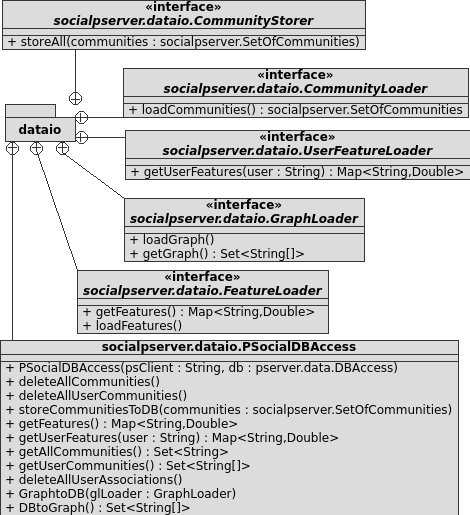
\includegraphics[scale=1.3]{Figures/dataIOClassDiagram.png}
	\rule{35em}{0.5pt}  % UnderLine figure	
	\caption[dataIOClassDiagram]{.dataIO Package classDiagram}
  %\end{center}	
  \label{fig:dataIOClassDiagram}  
\end{figure}

\clearpage

\subsection{Ανάκτηση - Αποθήκευση}
\label{Loaders - Storers}
\noindent
Για λόγους επεκτασιμότητας, στο πρόγραμμα είναι υλοποιημένα τα  \setlanguage{english} interfaces \textbf{Loaders - Storers}\setlanguage{greek}. Δίνουν στον κάθε προγραμματιστής 
την δυνατότητα να ανακτά και να αποθηκεύει δεδομένα από και σε όποιο μέσο θέλει. 
Για κάθε τύπου πληροφορία έχει υλοποιηθεί το αντίστοιχο \textbf{πρότυπο} το οποίο περιγράφει πως 
πρέπει να είναι μια κλάση χειρισμού του ανάλογου τύπου δεδομένων, 
στην οποία μπορεί να βασιστεί κάποιος και να προσθέσει τις απαραίτητες για αυτόν μεθόδους.\\

Πρότυπα:
\begin{description}
\item \textbf{CommunityStorer}   \hfill \\
  αποθηκεύει τις παραγόμενες κοινότητες, περιλαμβάνει τη μέθοδο:
\begin{lstlisting}[frame=single]
  public void storeAll(SetOfCommunities communities);
\end{lstlisting} 
\item \textbf{CommunityLoader}   \hfill \\
  ανακτά τις κοινότητες που έχουν είδη παραχθεί (χρησιμοποιείται για το Evaluation), περιλαμβάνει τη μέθοδο:
\begin{lstlisting}[frame=single]
  public SetOfCommunities loadCommunities();
\end{lstlisting} 
\item \textbf{GraphLoader}   \hfill \\
  ανακτά την πληροφορία φιλίας, περιλαμβάνει τις μεθόδους:
\begin{lstlisting}[frame=single]
  public void loadGraph();  \\ Load Graph in Memory
  public Set<String[]> getGraph();   // return Graph
\end{lstlisting} 
\item \textbf{FeatureLoader}   \hfill \\
  ανακτά όλα τα διαθέσιμα αντικείμενα της υπηρεσίας (χρησιμοποιείται για το Evaluation),
   περιλαμβάνει τις μεθόδους:
\begin{lstlisting}[frame=single]
  public Map<String, Double> getFeatures();
  public void loadFeatures();
\end{lstlisting} 
\item \textbf{UserFeatureLoader}   \hfill \\
  ανακτά τις προτιμήσεις κάθε χρήστη (αντικείμενα και αξιολογήσεις) (χρησιμοποιείται για το Evaluation), περιλαμβάνει τη μέθοδο:
\begin{lstlisting}[frame=single]
  public Map<String, Double> getUserFeatures(String user);
\end{lstlisting} 
\end{description}


\subsection*{Παράδειγμα χρήσης:}
\noindent
Για ανάκτηση της κοινωνικής πληροφορίας από την βάση Δεδομένων δημιουργούμε ένα αντικείμενο της κλάσης:\\ \setlanguage{english} \emph{GraphLoaderDB (implements GraphLoader)} \setlanguage{greek}\\
στο οποίο δίνεται ως παράμετρος ένα αντικείμενο DBAccess για να διαθέτει επικοινωνία με την Βάση.\\
Αντίστοιχα στην περίπτωση ανάκτησης του κοινωνικού γράφου από αρχείο, δημιουργούμε ένα αντικείμενο της κλάσης:\\
\setlanguage{english} \emph{GraphLoaderFile (implements GraphLoader)} \setlanguage{greek} \\
στο οποίο ως παράμετρος δίνεται η σχετική διεύθυνση του αρχείου. 
Παρόμοια διαδικασία ακολουθείται για όλες τις I/O κλάσεις.  



\subsection{DBAccess}
\label{DBAccess}

\noindent
Στην κλάση \textbf{PSocialDBAccess} είναι υλοποιημένες οι απαραίτητοι μέθοδοι για την
αλληλεπίδραση με την Βάση Δεδομένων.
Ένας από τους στόχους του socialPServer είναι η επέκταση του Pserver, 
 επομένως πρέπει να μπορεί να ανακτά και να αποθηκεύει δεδομένα που σχετίζονται 
  με τη λειτουργία του από την Βάση Δεδομένων του PServer.
Στην κλάση PSocialDBAccess βρίσκονται οι μέθοδοι που μεταφράζουν τις ανάγκες του προγράμματος για δεδομένα
  σε ερωτήσεις στην Βάση Δεδομένων του PServer.
  
Ποιο αναλυτικά, για πρόσβαση στην Βάση του PServer χρειάζεται ένα αντικείμενο \emph{pserver.data.DBAccess}.
Αυτό δίνεται ως παράμετρος στο πρόγραμμά μας και κατά την αρχικοποίηση δίνεται στην κλάση \emph{PSocialDBAccess}. 
Επίσης σαν παράμετρος δίνεται το όνομα του \emph{Πελάτη} (\emph{Client} του pServer) για τον οποίο γίνεται η διαδικασία. 
Πελάτης είναι η κάθε υπηρεσία η οποία ζητάει προσωποποίηση και πρέπει να είναι γνωστοποιημένη για να πραγματοποιηθούν επιτυχώς τα queries στη βάση,
 αφού ταυτοχρόνως ο pServer ενδέχεται να εξυπηρετεί πολλούς πελάτες. 

Κατά την υλοποίηση πρέπει να δοθεί προσοχή στις συνδέσεις που διατηρούνται 'ανοιχτές' με την Βάση γιατί μπορεί να δημιουργηθεί φόρτος στον δίαυλο επικοινωνίας.
Επομένως κατά την δημιουργία ενός αντικειμένου  \setlanguage{english} PSocialDBAccess \setlanguage{greek}:
ο Constructor αναλαμβάνει να ανοίξει και αμέσως να κλείσει μια πρώτη σύνδεση:\\\\


\begin{lstlisting}[frame=single]
  dbAccess.connect();
  dbAccess.disconnect();
\end{lstlisting}          
ώστε όλες οι μέθοδοι που θα ακολουθήσουν απλά να επανασυνδέονται:
\begin{lstlisting}[frame=single]
  dbAccess.reconnect();
\end{lstlisting}
και συνολικά το πρόγραμμα να διατηρεί μία μόνο σύνδεση με τη Βάση Δεδομένων.  


Για εγκατάσταση του socialPServer σε άλλο πρόγραμμα πρέπει να υλοποιηθεί η ανάλογη κλάση για επικοινωνία με τη Βάση (DBAccess)
  βασιζόμενη στις τωρινές μεθόδους.


\subsection{Loggers}
\label{Loggers}
\noindent
Καθ όλη την διάρκεια της λειτουργίας του, ο socialPServer δίνει μηνύματα τα οποία αποκαλύπτουν το στάδιο στο οποίο βρίσκεται η εκτέλεση,
τα βήματα που έγιναν ή ακόμα και τα λάθη που προέκυψαν.
Για την λειτουργική διαχείριση αυτών (output) χρησιμοποιούνται \emph{java Loggers} και συγκεκριμένα η default βιβλιοθήκη της java \emph{java.util.logging.Logger}.

Η διαδικασία Logging αποτελείται από τρία βασικά μέρη: \emph{Logger, Handler, Formatter}.
Έχουν υλοποιηθεί δύο σχετικές κλάσεις, η \textbf{LoggerInit} για τα πρώτα δύο και η \textbf{LoggerFormatter} για το τελευταίο.\\

Για την κάλυψη των αναγκών χρησιμοποιούνται δύο Loggers:\\
ο \textbf{socialPServerOutputLogger} ο οποίος θα αναλάβει όλο το output και το debugging του προγράμματος και ο\\
\textbf{algorithmOutputLogger} ο οποίος αφορά συγκεκριμένα την έξοδο των αλγορίθμων.

Στην κλάση \textbf{LoggerInit} η μέθοδος \textbf{initLogger} κάνει τις απαραίτητες αρχικοποιήσεις και ρυθμίσεις σχετικά με τους Loggers.
Σε πρώτο στάδιο καθορίζεται η θεμιτή \emph{ιεραρχία} των δυο Logger ώστε τα αλγοριθμικά μηνύματα να καταγράφονται αυτομάτως και στον socialPServerOutputLogger. 
\begin{lstlisting}[frame=single] 
  algorithmOutputLogger.setParent(socialPServerOutputLogger);
\end{lstlisting}

        
Στη συνέχεια καθορίζεται το \emph{output target} - \emph{Handler} που αντιπροσωπεύει το μέσω στο οποίο θα καταγράφονται τα μηνύματα. Εδώ προστέθηκαν δυο Handlers,
ένας για την εμφάνιση των μηνυμάτων στην \emph{κονσόλα} και ένας για την καταγραφή σε \emph{txt file} ώστε να είναι διαθέσιμα και μετά την εκτέλεση του προγράμματος.
\begin{lstlisting}[frame=single] 
  ConsoleHandler consoleHandler = new ConsoleHandler();
  fhAlgorithm = new FileHandler("./algorithmOutput.log");
  fhSocialPServer = new FileHandler("./socialPServerOutput.log");
\end{lstlisting}
  
Για την ομαλή λειτουργία αφού χρησιμοποιούνται καινούργιοι consoleHandlers πρέπει να απενεργοποιηθεί ο default Handler της java.
\begin{lstlisting}[frame=single] 
  LogManager.getLogManager().reset();
\end{lstlisting}

  
Επίσης καθορίζεται ποιος Handler αφορά ποιόν Logger:
\begin{lstlisting}[frame=single] 
  algorithmOutputLogger.addHandler(consoleHandler); // add consoleHandler
  algorithmOutputLogger.addHandler(fhAlgorithm);   // add FileHandler
  socialPServerOutputLogger.addHandler(fhSocialPServer);   // add FileHandler
\end{lstlisting}

